\section{Methods}
\label{sec:methods}

We study goal-directed non-prehensile pushing for a quadrupedal mobile manipulator under two contact modalities:
\textbf{Whole-Body (WB) pushing} using base/torso contact and \textbf{Arm-Mediated (AM) pushing} using the end-effector.
Both modalities are trained under an identical setting (same object/goal distributions, success metrics, and safety checks),
so differences in performance isolate the trade-offs introduced by the contact modality itself.

% =========================
% Task and MDP
% =========================
\subsection{Task and MDP}
\label{sec:mdp}
Each episode samples (i) an initial robot pose, (ii) a pushable object pose, and (iii) a goal region on the ground plane.
The objective is to reposition the object to the goal while maintaining object stability (no toppling) and avoiding unsafe robot--object contacts.
We formulate an MDP with simulator state $s_t$, observation $o_t$, action $a_t$, reward $r_t$, and termination conditions.
\paragraph{Success metric (pose + settling).}
Let $p_o(t)\in\mathbb{R}^2$ and $\psi_o(t)$ denote the object planar position and yaw at time $t$, and let $p_g\in\mathbb{R}^2$ and $\psi_g$ denote the goal pose.
We declare success when the object is within translation tolerance $\epsilon_{xy}$ and yaw tolerance $\epsilon_{\psi}$ for a dwell window of $K$ consecutive high-level steps,
while both the object and robot are near-stationary.

We compute the wrapped yaw error as
\begin{equation}
\label{eq:yaw_error}
e_{\psi}(t)\triangleq \left|\operatorname{atan2}\!\Big(\sin(\psi_o(t)-\psi_g),\,\cos(\psi_o(t)-\psi_g)\Big)\right|.
\end{equation}
The per-step success indicator is
\begin{equation}
\label{eq:succ_step}
\mathbf{1}_{\text{succ}}(t)=
\mathbf{1}\!\Big[
\big(\|p_o(t)-p_g\|_2<\epsilon_{xy}\big)\ \wedge\ \big(e_{\psi}(t)<\epsilon_{\psi}\big)
\Big],
\end{equation}
and during the dwell window we additionally require $\|v_o(t)\|_2<\epsilon_v$ and $\|v_r(t)\|_2<\epsilon_r$,
where $v_o(t)$ and $v_r(t)$ are the object and robot base linear velocities.
We declare episode success if $\sum_{i=t-K+1}^{t}\mathbf{1}_{\text{succ}}(i)=K$.


\paragraph{Stability and safety.}
We monitor object stability using an uprightness score based on the alignment between the object’s local ``up'' axis and world gravity.
Let $\hat z_o(t)$ be the unit vector of the object’s local $z$-axis expressed in the world frame, and let $\hat z_w=[0,0,1]^\top$ denote the world up direction.
We define
\[
\cos\theta(t) \triangleq \hat z_o(t)^\top \hat z_w,
\]
and terminate an episode as a \emph{topple} if $\cos\theta(t) < \cos\theta_{\min}$ (equivalently, if the tilt angle exceeds a fixed threshold).

Safety is enforced by monitoring robot--object contacts. For \textbf{AM}, we define an \emph{allowed} contact set consisting of the designated end-effector links
and treat contacts on all other robot bodies (e.g., base, legs, sensors) as \emph{non-permitted}. Non-permitted contacts are penalized and may trigger termination
if their impulse/force exceeds a threshold. For \textbf{WB}, we analogously specify an intended body-contact region and discourage hazardous contacts outside this region.
We report contact and safety outcomes (e.g., non-permitted impulses, illegal contacts, topples, emergency stops) in Sec.~\ref{sec:results}.

% =========================
% Hierarchical control
% =========================
\subsection{Hierarchical control and action spaces}
\label{sec:control}
Both modalities use a two-level hierarchy in the spirit of locomotion/loco-manipulation priors:
a high-level policy outputs compact task commands at low frequency, and a pretrained low-level controller tracks these commands to produce joint-level targets.
This separation stabilizes training by preventing task exploration from destabilizing gait and posture.

\paragraph{Low-level prior (shared).}
Learning pushing end-to-end is challenging because the policy must simultaneously discover (i) dynamically stable locomotion and (ii) task-directed contact behaviors.
In practice, exploration that is useful for learning pushing can destabilize gait, while stabilization objectives can dominate the learning signal.
We therefore adopt a hierarchical structure in which a \emph{frozen} low-level controller provides robust stabilization, and a high-level policy learns task decisions on top,
following the locomotion/loco-manipulation prior philosophy in \cite{Kumar2021RMA,2025relic}.

\textbf{Arm-mediated (Spot + arm).}
We pretrain a Spot locomotion prior in simulation while the arm executes randomized motions that induce disturbances.
Concretely, at training time the end-effector is commanded to track randomly resampled 3D targets (Fig.~\ref{fig:lowlevel_relic_training});
targets are updated online, and an IK/PD tracker enforces joint limits.
This produces a wide distribution of arm configurations and interaction-relevant perturbations that the base must reject.
After pretraining, the resulting locomotion policy is \emph{frozen} and used as the stabilizing layer in all AM pushing experiments.


\begin{figure}[h]
    \centering
    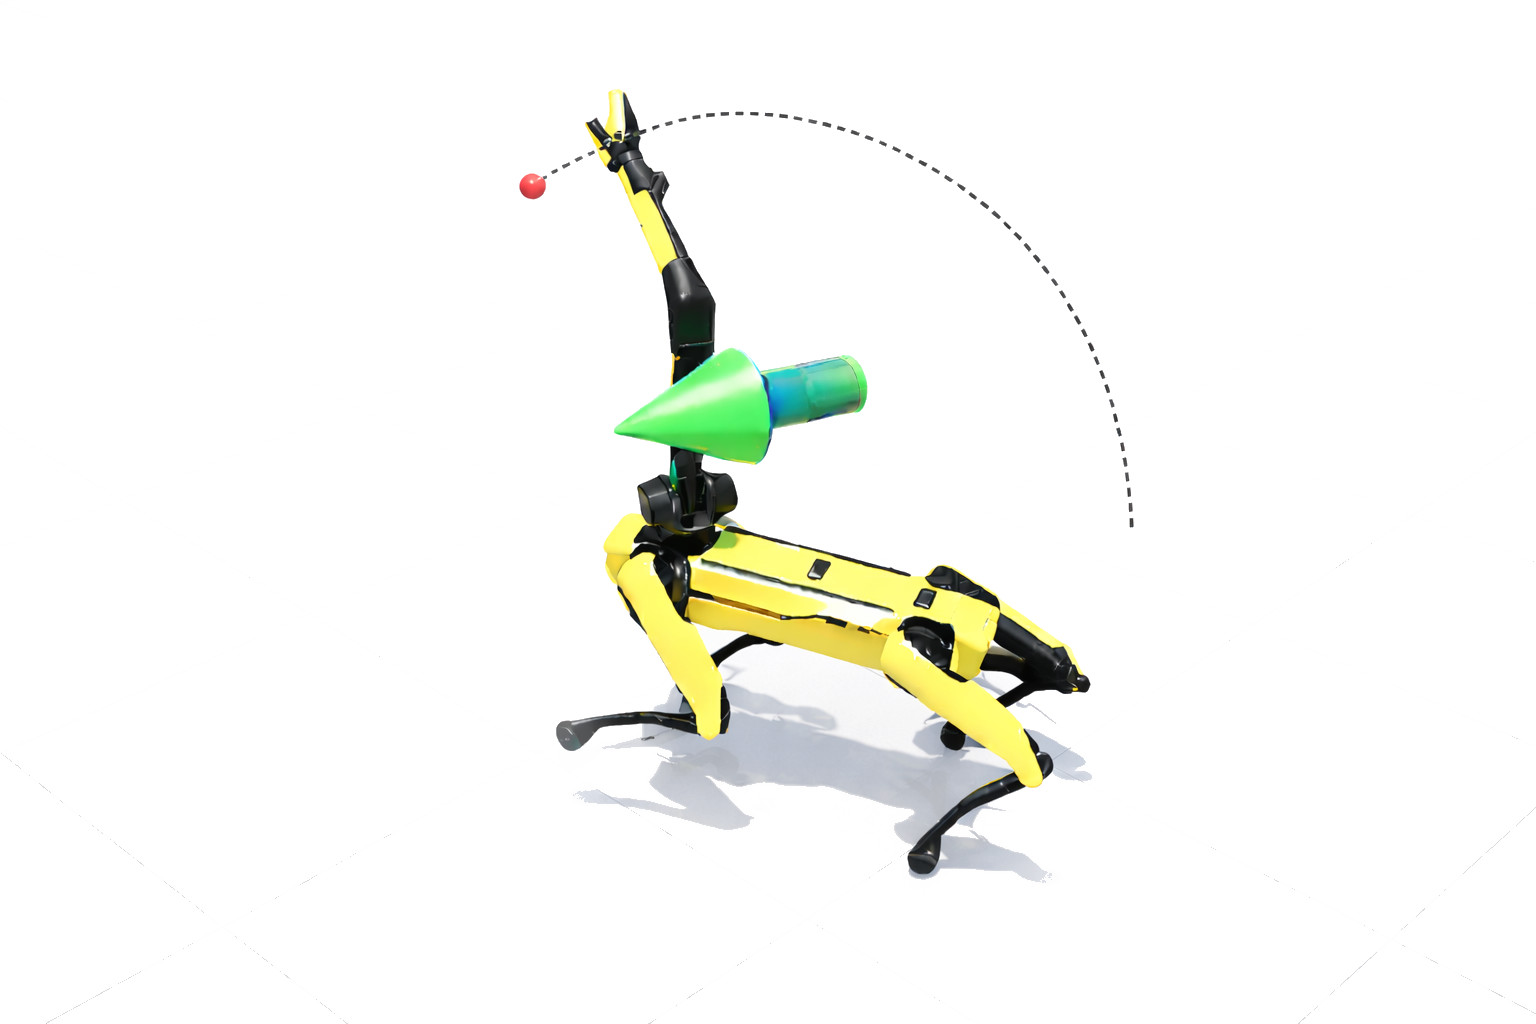
\includegraphics[width=\linewidth]{Images/relic.pdf}
    \caption{\textbf{Low-level locomotion prior pretraining.}
    Spot is trained to locomote while the arm tracks randomly resampled 3D end-effector targets (red), producing diverse arm motions and disturbances; the resulting locomotion policy is then frozen and used as a stabilizing prior for pushing.}
    \label{fig:lowlevel_relic_training}
\end{figure}


\textbf{Whole-body (WB).}
For WB, we use a standard pretrained quadruped locomotion policy that tracks commanded planar base velocities, trained with massively parallel RL in simulation
as in prior work \cite{Rudin2021WalkMinutes}. This policy is kept frozen during pushing and serves as the low-level stabilizer for all WB experiments.







\paragraph{WB action space (base-only).}
For whole-body pushing, the high-level policy outputs a planar base command
\begin{equation}
a_t^{\text{WB}} = [v_x,\ v_y,\ \omega_z],
\end{equation}
expressed in the robot body frame.
The frozen locomotion prior tracks this command and produces joint targets at the low-level control rate.
This keeps the high-level interface minimal and emphasizes contact planning through base motion.

\paragraph{AM action space (whole-body + arm).}
For arm-mediated pushing, the high-level policy outputs a compact whole-body command combining base motion, body regulation, and arm targets:
\begin{equation}
a_t^{\text{AM}} = \Big[
v_x,\ v_y,\ \omega_z,\ \phi,\ \theta,\ h,\ q^{\text{arm}}_{1:6}
\Big],
\end{equation}
where $(\phi,\theta,h)$ denote body roll/pitch/height targets and $q^{\text{arm}}_{1:6}$ are commanded arm joint targets.
The gripper DOF is kept fixed in our experiments (Spot is gripper-equipped), enabling future extensions to grasp-enabled interaction without changing the control stack.
A frozen loco-manipulation tracker converts these task commands into joint-level targets while maintaining base stability and safe arm configurations.

\paragraph{Control rates (fill once).}
We denote the high-level command rate by $f_{\text{HL}}$ and low-level control rate by $f_{\text{LL}}$ with decimation $d=f_{\text{LL}}/f_{\text{HL}}$.
All experiments use the same $(f_{\text{HL}},f_{\text{LL}},d)$ across modalities.

% =========================
% Our key novelty: interaction intent sampling + curriculum
% =========================
\subsection{Geometry-driven interaction intent sampling}
\label{sec:sampling}
A key challenge in arm-mediated pushing is that the policy must learn \emph{where} and \emph{how} to make contact on diverse objects.
To make interaction specification object-agnostic (and avoid hand-designed handles or per-object heuristics),
we introduce a geometry-driven interaction intent pipeline that samples a reachable, interaction-rich surface target each episode
and shapes exploration with a curriculum.

% =========================
% Fig: cached point-cloud target pipeline (one-column)
% =========================
\begin{figure}[t]
  \centering
  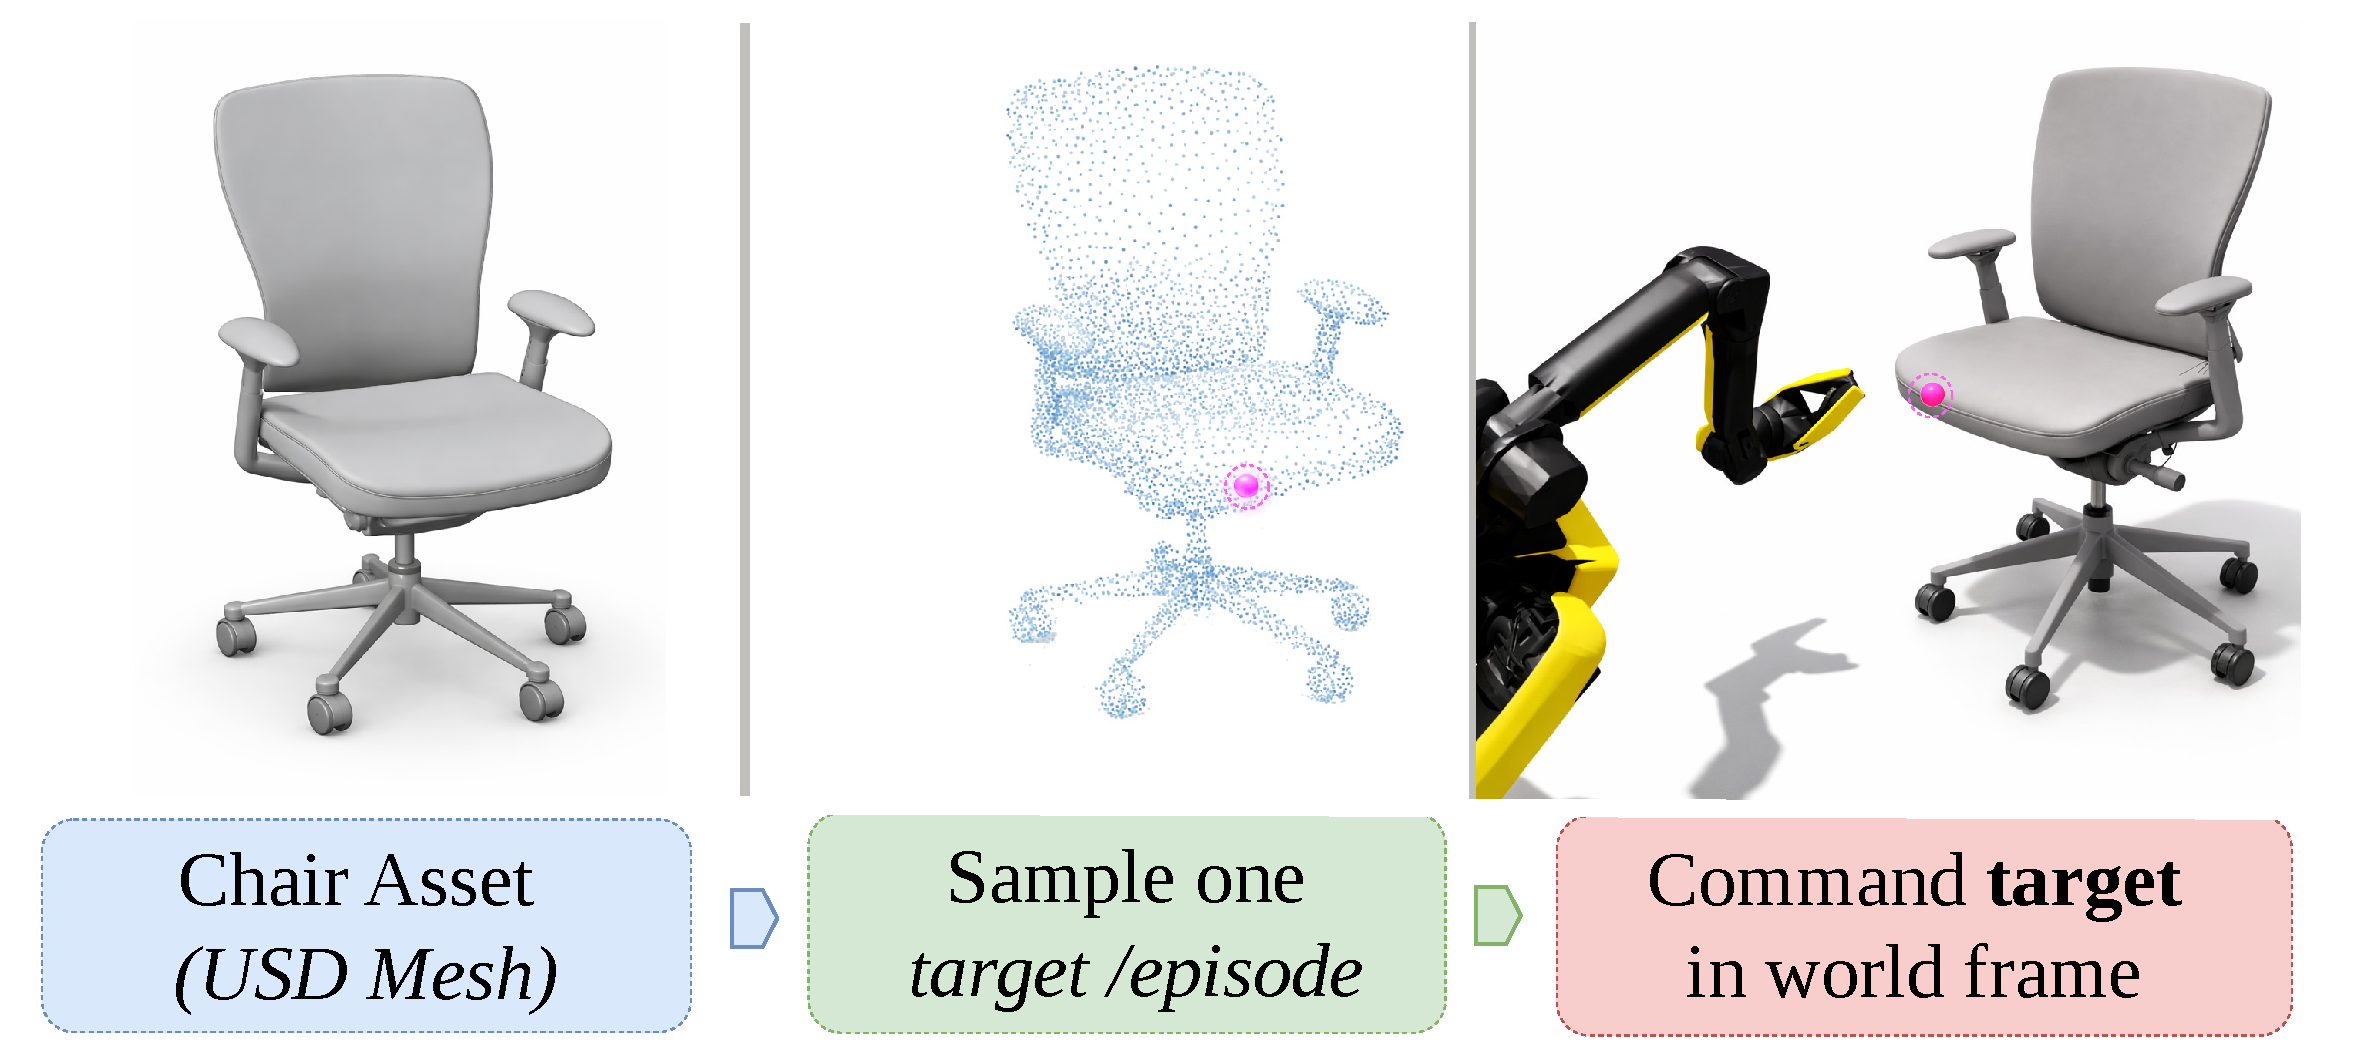
\includegraphics[width=\columnwidth]{Images/Sampling.pdf}
  \caption{\textbf{Interaction intent sampling.} For each object asset (e.g., chair), we cache a dense surface point cloud offline.
  At episode start, we filter the cloud to a reachable, interaction-rich subset and sample one target point $p_{\text{tgt}}$.
  The sampled point is transformed into the world frame and used as a reach/contact intent for AM.}
  \label{fig:chair_target_sampling_pipeline}
\end{figure}

\paragraph{Offline cached surface cloud.}
For each object mesh (USD asset), we precompute and cache a dense surface point cloud $\mathcal{P}$ once.
This amortizes geometry processing across training and supports large-scale randomization over object instances.

\paragraph{Interaction-rich filtering (object-agnostic).}
At episode initialization, we filter $\mathcal{P}$ to obtain $\mathcal{P}_{\text{int}}$ that emphasizes feasible and informative contacts.
Concretely, we keep points that satisfy:
(i) \textbf{reachability} under the current robot spawn and workspace bounds,
(ii) \textbf{clearance} (avoid points likely to cause immediate ground collision or degenerate contact),
and (iii) \textbf{interaction richness} (bias toward regions with larger usable surface area, e.g., broad planar faces rather than thin legs).
This reduces the contact discovery search space and yields consistent interaction intent across object families (boxes, cylinders, chairs).

\paragraph{Curriculum over interaction intents.}
We then apply a curriculum that gradually expands the difficulty of sampled intents.
Early in training, targets are sampled from an ``easy'' subset (high reachability and clearance); as competence increases,
sampling progressively covers the full $\mathcal{P}_{\text{int}}$ distribution.
This curriculum accelerates learning by first teaching reliable approach-and-contact, then training robust steering and correction under diverse contacts.

\paragraph{Reach intent as a command (AM only).}
For AM, the sampled target $p_{\text{tgt}}$ is used to form a reach/contact intent in the robot base frame and provides shaped guidance
that encourages the end-effector to establish contact at feasible locations while still optimizing the pushing objective.
WB does not use $p_{\text{tgt}}$ and must discover effective contact purely through base motion.

% =========================
% Observations
% =========================
\subsection{Observations}
\label{sec:obs}
Observations are designed to (i) express task geometry in the robot frame, (ii) provide proprioception for stable closed-loop behavior,
and (iii) support generalization analysis via optional privileged signals. Tables~\ref{tab:obs_wb} and~\ref{tab:obs_am} summarize the high-level policy inputs.

\paragraph{WB observations.}
WB uses compact planar task geometry and object motion:
robot/base state (velocities, projected gravity), robot--object vector, object--goal vector, distance-to-goal, object/goal headings,
and planar object velocity decomposed into goal-parallel and tangential components.
This supports ``push-from-behind'' behaviors and near-goal precision.


% =================================
% WB observation table (grouped)
% ================================
\begin{table}[h]
\centering
\caption{\textbf{WB policy observations (high-level).}}
\label{tab:obs_wb}
\footnotesize
\setlength{\tabcolsep}{3pt}
\renewcommand{\arraystretch}{1.08}
\begin{tabular}{l c}
\toprule
\textbf{Observation term} & \textbf{Dim.}\\
\midrule
% \multicolumn{2}{l}{
% \textit{Robot base state}}\\
Base linear velocity ($v_{\text{base}}$) & 3\\
Base angular velocity ($\omega_{\text{base}}$) & 1\\
Projected gravity ($g_{\text{base}}$) & 3\\
Previous action ($a_{t-1}$) & 3\\
\addlinespace[0.25em]\hline\addlinespace[0.15em]
% \multicolumn{2}{l}{\textit{Task geometry (planar)}}\\
Robot--object relative vector (xy) & 2\\
Object--goal relative vector in base frame (xy) & 2\\
Object--goal distance ($d_{bg}$) & 1\\
Pushable heading in base frame & 2\\
Goal heading in base frame & 2\\
\addlinespace[0.25em]\hline\addlinespace[0.15em]
% \multicolumn{2}{l}{\textit{Object motion (planar)}}\\
Object planar velocity in base frame (xy) & 2\\
Speed toward goal ($v_{\parallel g}$) & 1\\
Tangential speed ($v_{\perp g}$) & 1\\
\addlinespace[0.25em]\hline\addlinespace[0.15em]
\textit{Low-level prior (frozen): locomotion-policy obs} & 48\\
\bottomrule
\end{tabular}
\end{table}


\paragraph{AM observations.}
AM augments WB features with arm and end-effector geometry:
arm joint positions/velocities, end-effector--to--object vector, and relative object/goal orientation features.
This additional structure is required for contact placement, contact timing, and fine steering via the arm.

\paragraph{Privileged encoder.}
To study generalization and enable deployment-oriented distillation, we optionally include a privileged embedding
(e.g., object physical parameters or compact object descriptors available in simulation) during training.
This privileged signal can supervise an object-conditioned encoder used at test time, following an RMA-style teacher/student pattern.

% ==========================
% AM observation table (grouped)
% ============================
\begin{table}[t]
\centering
\caption{\textbf{AM policy observations (high-level).}}
\label{tab:obs_am}
\scriptsize
\setlength{\tabcolsep}{3pt}
\renewcommand{\arraystretch}{1.08}
\begin{tabular}{l c}
\toprule
\textbf{Observation term} & \textbf{Dim.}\\
\midrule
% \multicolumn{2}{l}{
% % \textit{Robot base + arm state}
% }\\
Base linear velocity ($v_{\text{base}}$) & 3\\
Base angular velocity ($\omega_{\text{base}}$) & 3\\
Projected gravity ($g_{\text{base}}$) & 3\\
Arm joint positions (relative) & 6\\
Arm joint velocities & 6\\
Previous action ($a_{t-1}$) & 9\\
\addlinespace[0.25em]\hline\addlinespace[0.15em]
% \multicolumn{2}{l}{
% % \textit{Task geometry (3D)}
% }
End-effector to object vector in base frame & 3\\
Object to goal vector in base frame & 3\\
Object rotation matrix in base frame ($R_{bo}$) & 9\\
Goal rotation in object frame ($R_{og}$) & 9\\
\addlinespace[0.25em]\hline\addlinespace[0.15em]
Privileged encoder & 16\\
\bottomrule
\end{tabular}
% \vspace{-0.8em}
\end{table}













% =========================
% Rewards + safety constraints
% =========================
\subsection{Reward design and safety constraints}
\label{sec:reward}
Both modalities use reward shaping that reflects three goals: (i) task completion (pose error and progress),
(ii) stability (upright and controlled motion), and (iii) safety (discourage undesired contacts).




\paragraph{WB reward}
WB combines goal progress and stable approach geometry with near-goal precision and settling.
We reward reduction in object--goal distance, discourage orbiting by biasing the robot to push from behind (relative to the goal direction),
and add a near-goal precision term together with a dwell-based success bonus to enforce stable placement rather than transient crossings.
We further penalize loss of uprightness (to discourage tipping) and regularize action changes to reduce jitter and improve robustness.
Concretely, we use a shaped WB reward written as a weighted metric vector:
\begin{equation}
\footnotesize
\label{eq:wb_reward_condensed}
r_t^{\mathrm{WB}}=
\Big\langle
w^{\mathrm{WB}},
\begin{bmatrix}
\clip\!\big(d_{bg}(t\!-\!1)-d_{bg}(t),-\delta,\delta\big)\\[0.1em]
\big(\max(0,-\hat u_{rb}(t)^{\!\top}\hat u_{bg}(t))\big)^2\\[0.1em]
\exp\!\big(-d_{bg}(t)^2/\sigma_{xy}^2\big)\ +\ \mathbf{1}\!\Big[\sum_{i=t-K+1}^{t}\mathbf{1}_{\text{succ}}(i)=K\Big]\\[0.1em]
\clip\!\big(\cos\theta(t),0,1\big)\ -\ \mathbf{1}\!\big[\cos\theta(t)<\cos\theta_{\min}\big]\\[0.1em]
-\|a_t-a_{t-1}\|_2^2
\end{bmatrix}
\Big\rangle ,
\end{equation}
\noindent where $w^{\mathrm{WB}}$ is a fixed weight vector that balances progress, approach geometry, precision/settling, stability, and smoothness.




\paragraph{AM reward}
AM uses a pose-matching objective (we use a keypoint-based pose error for robustness to contact mode changes),
plus a reach shaping term that encourages the end-effector toward the sampled intent $p_{\text{tgt}}$.
We additionally penalize undesired contacts on non-permitted bodies and regularize action rates for smooth, safe behaviors.





% ---------------- AM reward terms (style-matched) ----------------
% \subsubsection{Arm-mediated pushing reward structure.}
\begin{table}[h]
\centering
\caption{\textbf{Arm-mediated pushing (AM): reward terms.}}
\label{tab:am_reward_terms}
\scriptsize
\setlength{\tabcolsep}{3pt}
\renewcommand{\arraystretch}{1.10}
\begin{tabular}{@{}p{2.0cm}p{\dimexpr\columnwidth-2.0cm-0.55cm-4\tabcolsep\relax}p{0.55cm}@{}}
\toprule
\textbf{Term} & \textbf{Definition} & \textbf{$w$}\\
\midrule
\multicolumn{3}{@{}l}{\textit{Goal pose + progress}}\\
Pose match &
$r_{\text{pose}}=\exp\!\big(-e_{\text{kp}}^{2}/\sigma_3^{2}\big)$
& 3.0\\
Reach shaping &
$r_{\text{reach}}=\exp\!\big(-\|p_{ee}-p_{\text{tgt}}\|^{2}/\sigma_1^{2}\big)$
& 2.5\\
Velocity to goal &
$r_{\text{vel}}=\exp\!\big(-(1-\alpha)^{2}/\sigma_2^{2}\big)$
& 0.156\\
\addlinespace[0.20em]\midrule\addlinespace[0.10em]
\multicolumn{3}{@{}l}{\textit{Stability + safety}}\\
Object stability &
$r_{\text{stab}}=\sigmoid\!\big(s(\cos\theta-\cos\theta_{\lim})\big)$
& 0.4\\
Undesired contacts &
$r_{\text{col}}=-\sum_{b\in\mathcal{B}_{\neg ee}}\mathbf{1}\!\left[\|F_b\|>\tau\right]$
& -0.05\\
\bottomrule
\end{tabular}
\end{table}




% \paragraph{Contact constraints.}
AM explicitly distinguishes allowed contact links (end-effector) from disallowed bodies (base, legs, sensors, etc.).
We penalize contact impulses on disallowed bodies and optionally terminate episodes on large violations.
This ensures a clean comparison of contact modality: AM is trained to localize contact through the arm rather than relying on the base.



% =========================
% Training + Randomization (brief; full specs in Experiments)
% =========================
\subsection{Training and randomization (summary)}
\label{sec:training_summary}
We train WB and AM with PPO in GPU-parallel Isaac Lab simulation. Both modalities use the same rollout horizon, termination conditions, and success metric.
They differ only in (i) the high-level \emph{action interface} (Sec.~\ref{sec:control}), (ii) the \emph{observation design} (Sec.~\ref{sec:obs}),
and (iii) the \emph{permitted-contact constraints} used for safety monitoring (Sec.~\ref{sec:reward}).

To promote generalization, we apply domain randomization over object dynamics and initial conditions (e.g., mass, friction, CoM offsets, and spawn/goal sampling),
and enforce clearance constraints at reset to avoid trivial penetrations. We train with PPO using the default hyperparameter settings provided by the RSL-RL library
\cite{schwarke2025rsl}. All remaining numerical settings for the experimental protocol (e.g., $N_{\text{env}}$, episode horizon, control rates, and randomization ranges)
are reported in Sec.~\ref{subsec:exp_setup} and Tables~\ref{tab:setup_summary}--\ref{tab:domain_rand}.